\documentclass[conference]{IEEEtran}
\IEEEoverridecommandlockouts
% The preceding line is only needed to identify funding in the first footnote. If that is unneeded, please comment it out.
\usepackage{cite}
\usepackage{amsmath,amssymb,amsfonts}
\usepackage{algorithmic}
\usepackage{graphicx}
\usepackage{textcomp}
\usepackage{xcolor}
\def\BibTeX{{\rm B\kern-.05em{\sc i\kern-.025em b}\kern-.08em
    T\kern-.1667em\lower.7ex\hbox{E}\kern-.125emX}}
\begin{document}

\title{A survey of software architectural patterns\\
{\footnotesize \textsuperscript{*}}
\thanks{Identify applicable funding agency here. If none, delete this.}
}

\author{\IEEEauthorblockN{Abhijit Taware}
\IEEEauthorblockA{\textit{Computer Science (Masters student)} \\
\textit{UNB}\\
Fredericton, Canada \\
ataware@unb.ca}
\and
\IEEEauthorblockN{Luigi Benedicenti}
\IEEEauthorblockA{\textit{ Computer Science (Dean)} \\
\textit{UNB}\\
Fredericton, Canada \\
luigi.benedicenti@unb.ca}
}

\maketitle

\begin{abstract}
With the advent of paradigm like microservices, containerized applications, cloud computing etc., the software developement process is being influenced heavily. This helped evolve the software developement and triggered the emergence of new architectural patterns. In this document, the common software architectural patterns are brifely discussed. The document further describes latest advancements in service oriented architecture, microservices, reactive programming and resilient software development. A case study is given to find existing patterns in the application and possible future enhancements.
\end{abstract}

\begin{IEEEkeywords}
SOA, microservice, reactive programming, resilient software
\end{IEEEkeywords}

\section{Architectural design patterns}
Large enterprise needs software that scales with ever changing and increasing needs of the business. Selecting the right architecture before diving into the real work is crucial to the success of the application and enterprise. This section explores various architectural patterns used in the industry. The pros and cons are discussed for each of the pattern.

\subsection{Layered architecture}
It is the most common architecture style, that organize similar modules into horizontal layers. The layers are independent of others and interact using exported APIs. An application can be designed using any number of layers. The network protocol stack is a good example of layered architecture. The in upper layer is transmitted to lower layers using encapsulated packets. A layer don't have to know the inner working of other layer and communication happens through a set of APIs exposed by each layer. Another example of business application, that is divided into presentation, logic and data tiers. Following of some of the benefits offered by this architecture.
\begin{itemize}
\item Layers can be developed and tested independently.
\item Changes made in one layer doesn't affect the other layer, hence maintainable.
\item Low coupling and high cohesion
\item Lower layers have no dependency on higher layer and hence reusable.
\end{itemize}

The disadvantages can be summarized as follows.
\begin{itemize}
\item A change to any component may trigger a redeployment of the entire application.
\item Each layer can have separate physical deployment or an entire application can be replicated. It is too coarse grained from deployment perspective.
\item Communication across layers can be a performance bottleneck for certain applications.
\end{itemize}

\subsection{client-server architecture}
It consists of a server and multiple clients. The server keeps listening to the client requests. The server responds to any new client requests i.e., provides a service to those clients.
E.g. the encryption key control server \cite{hytrust} provides encryption keys to the requesting clients over network. This model is prone to denial of service attack. The scalability requires replicating the server components with load balancing, failover and failback mechanisms.
\subsection{Pipe and filter architecture} 
This approach is suitable for large applications that can be broken down to multiple steps. Each step refers to a filter. The filter applies a specific function to the data and can work asynchronously as well. The pipes refer to the connectors between these filters. The output of one filter serves as an input for the next filter on the pipeline. The common example is Unix pipes. 
\begin{itemize}
\item Adding a new step is easy by adding a new filter and adding it to existing pipe stream.
\item It is easier to reuse of filters doing generic actions.
\item Promotes concurrency of different filters do not depend on each other.
\item The errors gets propagated across the filters, which is a downside of this architecture.
\item A broken filter leads to a complete broken pipe.
\end{itemize}

\subsection{Peer to peer architecture}
A peer-to-peer (P2P) architecture \cite{peer2peer} consists of a decentralized network of peers i.e. nodes. Unlike client-server architecture, a node in this architecture can act both as a server and a client. The workload is split into small chunks that can be reassembled later, allowing peers to work simultaneously on a task. E.g. P2P file sharing, where a file is split into chunks that allows many chunks to be downloaded from different peers at the same time.
\begin{itemize}
\item Need for centralized server is eliminated.
\item There is no single point of failure, unless the number of peers are too few.
\item The increase in number of peers can be handled easily i.e., scalable.
\item The model is prone to security issue, as an infected peer can affect the whole network.
\item Fairness guarantees are difficult to enforce as many leeches could benefit free riders.
\item Instant messaging, file sharing, collaboration apps use P2P architecture. E.g. Bitcoin, BitTorrent, napster etc.
\end{itemize}

\subsection{Event based architecture}
The callbacks mechanism describes this architecture well. It consists of source, listener, and a bus. The event source send a message i.e. an event on the bus to other component. The listener responds by performing some action. The components communicate only via the event bus. The linux device driver interrupt handlers employ this mechanism. 
\begin{itemize}
\item Changing name or type of an even requires changes to the listener.
\item Too many event sources or listeners lead to bottleneck for the bus.
\item Following the control flow is difficult due to asynchronous nature of events.
\item The producer and consumer of the event need not be aware of each other allowing for loose coupling
\item Loose coupling makes it easy for a component to evolve independently.
\item Message passing over the bus introduce additional abstraction and may not be efficient.
\end{itemize}

\subsection{Interpreter}
It consists of a program to be executed, an interpreter which runs such a program, program state and memory component required any storage needs. The interpreted languages like Awk, Perl, Python or Java are prime example of this architectural style of development.
\begin{itemize}
\item Program development becomes easy with the help of interpreter.
\item Allows portability across various platforms.
\item Debugging become easier.
\item An extra level of indirection makes execution slower.
\item Interpreter can guard against malicious instruction 
\end{itemize}

\subsection{Blackboard}
It is similar to boardroom where people solve the problem using a whiteboard. The component blackboard acts as a global information store. It allows various components to collaborate towards the final solution. The controller component monitors the blackboard and schedules individual knowledge sources. The knowledge sources are specialized workers with its own representation of the problem. The communication happens through the blackboard. The CAD software is an example of blackboard design.
\begin{itemize}
\item Efficient scheduling of tasks and resource management across a distributed network.
\item Better suited when a problem can be split into multiple sub-problems.
\item Not always easy to break down a task into subproblems.
\item Everything is shared and can cause unwanted information flows.
\item Controller design can become overly complex and unmaintainable.
\item Knowledge sources being independent, allows for reusability.
\end{itemize}

\subsection{Microkernel Architecture}
Microkernel \cite{microkernel} is a typical Operating System architecture. Minix \cite{minix} is a good example for this. The idea is to keep the core minimal functionality in kernel. The platform dependent code can be implemented as internal servers, e.g. device drivers. It might consist of few external servers for additional functionality like file-systems, memory management etc. Applications interact via adapter, which is a glue between external servers and the applications. This allows changing external servers without affecting applications.\par
The userland applications like eclipse editor is a simple example of microkernel architecture. Minimal functionality is provided by the basic package. Additional plung-ins make it feature rich and production ready. Similarly the internet browser is an example of this pattern which mainly uses plung-ins to enhance functionality.

\section{New architectural styles}
The monolithic applications causes lot of bloated code with dependencies and slower deployment cycles. This also leads to more buggy applications.
All such issues leads to newer architectural paradigm shift, which is described in the following subsections. Following patterns are discussed exclusively in this context.
\begin{itemize}
\item Service Oriented architecture (SOA)
\item Microservices
\item Containers
\item Reactive programming
\item Resilient software development
\end{itemize}

\subsection{SOA}
SOA \cite{SOA} allows application to be modularized into services. A centralized component is responsible for the service integration and communication.
This is achieved using an Enterprise service bus (ESB), which acts as an \textit{orchestrator}. The data model for SOA applications evolve by an agreement between many services.
However, such a canonical data model being shared by many services, which limits the evolution. The services often reflect the communication pattern of the organization, a.k.a. Conway's law \cite{conway}. Figure \ref{soaBlockDiagram} depicts the SOA block diagram.

\begin{figure}[htbp]
\centerline{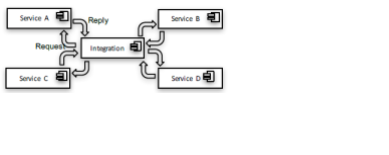
\includegraphics[scale=0.4]{SOA.png}}
\caption{SOA block diagram.}
\label{soaBlockDiagram}
\end{figure}

\par The SOA is often implemented as web services which use following communication methods.
\begin{itemize}
\item Simple Object Access Protocol (SOAP) for synchronous communication with other web services, typically over HTTP. Components that use SOAP are often described in a Web Services Description Language (WSDL). The WSDL is an XML-based interface description language that is used for describing the functionality offered by a web service. 
\item The REpresentational State Transfer (REST) protocol too can be used for basic request/response operations between the services.
\end{itemize}

Most organizations need to deal with existing legacy applications before adopting the SOA architecture. The key business processes depend on such legacy systems and hence a step by step solution must be adopted to move towards SOA. Following are some of the options strategies to deal with the change.
\begin{itemize}
\item Use commercial off the shelf components to replace existing system. This can be more costly in future.
\item Wrap the current legacy system with a middleware that can offer the legacy system interface through a Web service.
\item Redevelop the legacy application to achieve the optimal levels of decoupling. However, legacy code can be complex and lack of documentation could make it more challenging.
\end{itemize}
SOA sometimes is referred to as "simple service and smart pipes" \cite{comparison}.
\subsection{Microservices}
Microservices \cite{microservice} allows applications to be made up of small, self-contained independent units i.e., services working together through APIs interface. Martin fowler \cite{microservice} describes following key characteristics for of the microservice.
\begin{itemize}
\item \textit{Componentization} : Services are independent units that communicate with other services using web requests or remote procedure calls.
\item \textit{Business capabilities} :  Services represent the business capability, with responsibility for a complete stack.
\item \textit{Product rather than projects} : Microservices treat services as products and claim ownership. The ongoing maintainance requires complying with business needs.
\item \textit{Dumb pipes and smart endpoints} : Microservices do not use ESBs. The services are intelligent and communication channel is userd merely for message passing. The communication channel does not implement any service functionality i.e., the channel implementation is simple.
\item \textit{Decentralized governance} : There is no orchestrator, instead it evolves towards choreography and event collaboration.
\item \textit{Bounded context} : Domain-driven design complex domain up into multiple bounded contexts and maps out the relationships between them. This leads each service to have its own localized version of data model promoting loose coupling.
\end{itemize}
Figure \ref{soaBlockDiagram} depicts the SOA block diagram.

\begin{figure}[htbp]
\centerline{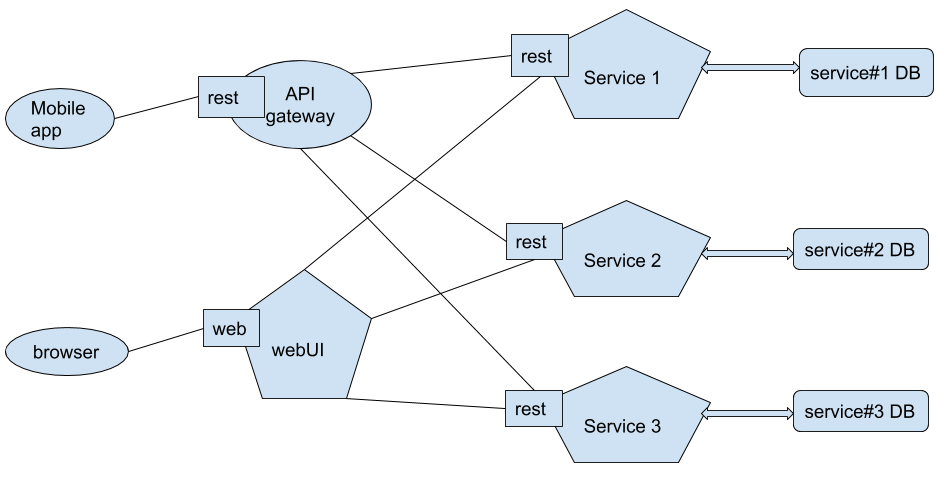
\includegraphics[scale=0.25]{Microservice.png}}
\caption{Microservice block diagram.}
\label{Microservice}
\end{figure}

Microservices architecture constantly introduce new services that requires DevOps to ensure component updates in production environment. 
It has disadvantages such as code duplication, interfaces mismatch, operations overhead and the challenge of continuous testing of multiple systems. However, the benefits of creating loosely coupled components by independent teams using a variety of languages and tools far outweigh the disadvantages. Some of examples of microservice adoption are listed below.

\begin{itemize}
\item \textit{Netflix} : Moved away from single war file to full fledged microservice approach.
\item \textit{The gaurdian} : This website maintains their core monolithic system but use microservice for new components.
\item \textit{Gilt groupe} : Uses massive microservice approach to their shopping site, allowing various teams working on different services.
\end {itemize}

\subsection{Containers}
Containers \cite{lxc} \cite{kubernetes} are often termed as light weight virtual machines. An example is lxc containers built for linux systems. They provides an isolated environment with exclusive access to resources like memory, network, storage etc. The following components enable the containers to provide isolation and bare-metal performance. Figure \ref{containerBlockDiagram} shows block diagram of the containers.

\begin{figure}[htbp]
\centerline{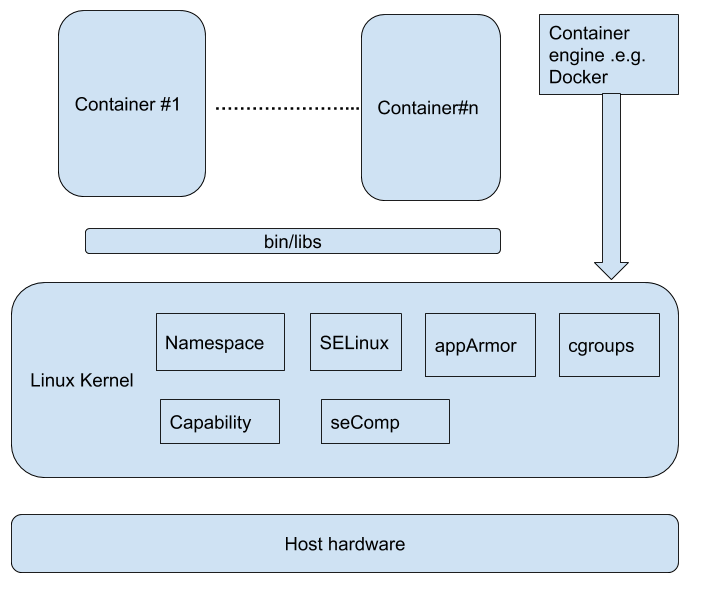
\includegraphics[scale=0.3]{container.png}}
\caption{Container block diagram.}
\label{containerBlockDiagram}
\end{figure}

\begin{itemize}
\item \textit{Kernel namespaces} --- A namespace wraps a global system resource making it appear to the processes as their own isolated instance.
\item \textit{SELinux} --- provides access control
\item \textit{SeComp} --- restrict malicious usage of system calls
\item \textit{chroot} --- allows process to change root i.e., restricts process to specific directory structure.
\item \textit{Kernel capabilities} --- Distinguish between privileged  and un-privileged  process and allow access accordingly
\item \textit{CGroups} --- Limits, accounts for and isolates process resource usage.
\end{itemize}

The virtual machines (VM) are widely used to host the applications. A single physical machine can have multiple VMs running allowing for a service per instance. The virtual machines have their own operating system (OS) and are resource heavy. Contrast this with containers which share the kernel with the host OS and provide resource isolation equivalent to VMs. This makes containers more attractive to deploy the microservices. Container can be equipped to have its own IP address allowing it to be the best option in cloud environments like Amazon EC2. Nothing restricts one to create containers insides a VM hosted on a third party cloud. \par
The containerized applications need to account for failure too. It should have a mechanism to recover from failures, i.e., restarting the service on a different host or respawing the containers. 
Today the distributed system development, with microservice architectures built from containerized software components \cite{containerPatterns} is dominating the industry.

\subsection{Reactive programming}
Reactive programming (RP) is a new paradigm that deals with the data flows and the propagation of change. It is possible to express static or dynamic data flows with ease in the reactive programming languages, and that the underlying execution model will automatically propagate changes through the data flow. For example, in a model–view–controller (MVC) architecture, RP can facilitate changes in an underlying model that are reflected automatically in an associated view \cite{mvc}. \par
Traditionally such a task was achieved using observer pattern \cite{gof}. This pattern is mainly used to implement distributed event driven systems, consisting following characteristics.
\begin{itemize}
\item A "subject" and "observer" are the main objects.
\item Any change to subject is automatically propagated to the observers.
\item Observers should be registered with the subject to receive the change notification.
\item Subject maintains list of observers and calls update method on all of them in the event of change.
\end {itemize}
The observer pattern is criticized for lack of composability, inversion of the logical relation among reactive entities and limited readability \cite{observer}. Also, it can be a source of memory leaks especially when the observer object fails to unregister itself. During such a situation the observer object can not be garbage collected. \par

The following pseudocode \cite{reactive_walkthrough} illustrates the reactive paradigm well. This code snippet receives the mouse.clicked event and the current mouse.position .
\begin{enumerate}
\item clicked: Event = mouse.clicked
\item scaledPosition: Signal[(Int,Int)] = mouse.position X 0.5
\item lastClick: Signal[(Int,Int)] = \\
      clicked.snapshot(scaledPosition)
\end{enumerate}

The mouse position is scaled by 0.5 and saved to scaledPosition variable. On every mouse click, the snapshot of the position is saved to lastClick. Any change to mouse position will reflect to scaled position in conventional imperative programming language. Same is true about the lastClick variable. However, RP converts the line #2 into a constraint. The RP runtime identifies the dependency between scaledPosition and mouse.position, making realtime updates possible. This technique can be applied to MVC architecture to get the view updated every time something changes in the model. 
\begin{itemize}
\item There are no bugs because of forgotten updates
\item No redundant computations in case programmers code defensively and update too much,
\item Applications are easily extensible as constraints can be composed, i.e., built on top of other constraints.
\end{itemize}

\subsection{Resilient software development}
With the advent of cloud computing, microservices and containers technology, applications are growing exponentially. The providers need to account node failure is commonplace thing for such a large scale applications. The application failure directly translate into loss of revenue. Application developer must consider a good balance between the cost of being resilient \cite{Hornsby} and the possible loss of revenue. The resilience can be achieved using some of the following patterns, which are becoming more common place in software architectures nowadays.
\par \textit{Redundancy} : Increasing the availability by deploying several instances, possibly in different zones or regions, e.g. AWS availability zones.
\par \textit{Autoscaling} : Scaling the resources dynamically according to the demand as opposed to doing it manually is auto scaling. E.g. Amazon's gold AMI are pre-configured instances which can be deployed on demand. Another example is Dockerfile which helps get rid of configuration scripts and deploy containerized application automatically.
\par \textit{Infrastructure as code} : It is process of managing the computer data centers using configuration templates. It is also referred to as Infrastructure as a Service (IaaS). In the event like accidental deletion, templates provide quick way to recover the infrastructure. 

\par \textit{Immutable infrastructure} : Immutable components are replaced for every deployment, rather than being updated in place.
\begin{itemize}
\item No updates should ever be performed on live systems
\item Always start from a new instance of the resource being provisioned
\end{itemize}
Immutable infrastructure promotes canary deployment i.e., deployement to a smallest possible set. If the such deployement fails, immediate rollback is possible.

\par \textit{Stateless application} :
Autoscaling and immutable infrastructure requires the application to be stateless. The application must treat all the client requests independent of earlier requests. It should not store any information on disk or in memory. However, state sharing within the autoscaling group is conducted using in-memory caching mechanism like Redis, Memchached etc.

\par \textit{Cascading failures} :
A single failure can trigger multiple others failures impacting the availability. E.g. if an overloaded cluster goes down, the traffic would be redirected to another cluster. This in turn overloads the new cluster, causing more failures. Following techniques are employed to handle such failures.
\begin{itemize}
\item \textit{Timing out} faster may mean the service is degraded instead of failing.
\item Due to transient errors, clients may resend the same requests. Making such requests \textit{idempotent} can solve the failures.
\item \textit{Degradation} implies that instead of failing, your application degrades to a lower-quality service. It consist of service that is easier to compute and deliver to the user.
\item \textit{Dropping} un-important traffic should help certain failure cases.
\end{itemize}

\subsection{Case Study : Hytrust Data Control}
This section briefly explain the Hytrust Datacontrol \cite{hytrust} appliance and the architectural analysis is presented as well.
The UI, Keycontrol Server and encryption agents on client machines are three main components of the Hytrust appliance. Figure \ref{hytrustBlockDiagram} shows the various components and their interaction.
\begin{figure}[htbp]
\centerline{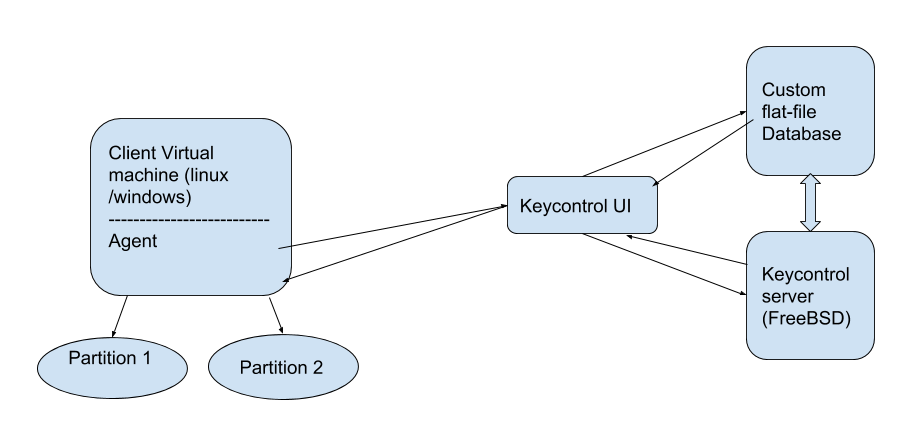
\includegraphics[scale=0.3]{HytrustAppliance.png}}
\caption{Hytrust data control block diagram.}
\label{hytrustBlockDiagram}
\end{figure}

The client agent requests the encryption keys from Keycontrol appliance using REST API. These keys are used to encrypt the client virtual machine (VM) partitions.
Client can do following actions:
\begin{itemize}
\item Create a set of Virtual machine i.e. CVMSet
\item Register/Unregister a VM in the CVMSet.
\item Encrypt/Decrypt a partition, applicable to registered VMs
\item Rekey the partition i.e. change the partition encryption key for security reasons.
\item Create a shared folder on AWS for all the VMs registered in a particular CVMset.
\item Add/remove files to shared folder with specific encryption keys.
\item CVMset have authorized user requiring the Keycontrol to implement access control.
\item User/Group creation/deletion is supported via UI.
\end{itemize}

\textit{Availability} is ensured by running two instances of the Keycontrol appliance in master-slave mode.
In case of failure the roles are switched for the master and the slave nodes. 
\par\textit{Consistency} of database is maintained by replicating the changes across the two node cluster. However, this is tightly coupled with the Keycontrol and errors are hard to debug. 
\par\textit{Load balancing} is achieved by allowing each client to support preferred node in the cluster, though initial registration should happen through active node only.
\par\textit{Caching} the keyid on client side for the files encrypted in the AWS cloud improves response time.
\par\textit{Autodeployment} is achieved by keeping the Golden AMIs for Keycontrol appliance.
\par\textit{Availability} can be truly enhanced by deploying the cluster nodes across different zone in Amazon/Azure/IBM cloud.
\par\textit{Content delivery network (CDN)} can be used to cache the static website content. It is useful especially when the client and the appliance belong to different availability zones.
\par Despite being a high performant appliance, the DB errors can lock-down the whole appliance and client becomes tainted. Microservices approach should be a real help here. The database should be divided into units as per business needs making it available to respective microservice i.e. webservice. Completely modularized server is hard to achieve, however the keycontrol can be divided into following components.
\begin{itemize}
\item UI component
\item User/Group creation/deletion
\item Encryption Key generation
\item CVMset creation/deletion
\item VM registration etc.
\end{itemize}

\par\textit{Testing} large applications is often a challenge. Simulating thousand of clients would require huge resources i.e., memory, cpu. However, containers can be configured to run the client agents and perform desired actions. Each container can be configured to have an IP and mac address to simulates actual client requests. Using Dockerfile will further simplify the process of testbed creation and automated tests.
\par Analyzing existing applications from architectural perspective truely opens up new alternatives for future designs. The long term benefits of getting architecturally correct model, makes the study of the software architecture more compelling.

\begin{thebibliography}{00}
\bibitem{microservice} J. Lewis and M. Fowler,Microservices-A definition of this new architectural term, 2014.  https://martinfowler.com/articles/microservices.html
\bibitem{comparison} Cerny, Tom & J. Donahoo, Michael & Pechanec, Jiri. (2017). Disambiguation and Comparison of SOA, Microservices and Self-Contained Systems. 228-235. 10.1145/3129676.3129682.
\bibitem{SOA}Gold, N.E., Knight, C., Mohan, A., & Munro, M. (2004). Understanding service-oriented software. IEEE Software, 21, 71-77.
\bibitem{caseStudy} Marquez, Gaston & Astudillo, Hernan. (2018). Actual Use of Architectural Patterns in Microservices-based Open Source Projects.
\bibitem{conway} M. Conway, Conways law. https://en.wikipedia.org/wiki/Conway
\bibitem{hytrust} Key Control Server.  https://www.hytrust.com/products/keycontrol/
\bibitem{lxc} LxC Containers.  https://linuxcontainers.org/lxc/introduction/
\bibitem{kubernetes} Kubernetes. https://kubernetes.io/
\bibitem{containerPatterns}Brendan Burns and David Oppenheimer. 2016. Design patterns for container-based distributed systems. In Proceedings of the 8th USENIX Conference on Hot Topics in Cloud Computing (HotCloud'16). USENIX Association, Berkeley, CA, USA, 108-113.
\bibitem{mvc}Model-View-Controller and the Observer Pattern http://peak.telecommunity.com/DevCenter/Trellis#model-view-controller-and-the-observer-pattern
\bibitem{gof} Erich Gamma, Richard Helm, Ralph Johnson, John Vlissides (1994). Design Patterns: Elements of Reusable Object-Oriented Software. Addison Wesley. pp. 293ff. ISBN 0-201-63361-2.
\bibitem{observer} Maier, Ingo et al. “Deprecating the Observer Pattern.” (2010).
\bibitem{reactive_walkthrough} G. Salvaneschi, A. Margara and G. Tamburrelli, "Reactive Programming: A Walkthrough," 2015 IEEE/ACM 37th IEEE International Conference on Software Engineering, Florence, 2015, pp. 953-954. 
\bibitem{Hornsby} Adrian Hornsby, Patterns for resilient architecture, https://aws.amazon.com/developer/community/evangelists/adrian-hornsby/
\bibitem{microkernel} Jorrit N. Herder , TOWARDS A TRUE MICROKERNEL OPERATING SYSTEM, http://www.minix3.org/theses/herder-true-microkernel.pdf
\bibitem{minix} The minix OS. https://www.minix3.org/
\bibitem{hytrust} Hytrust Datacontrol. https://www.hytrust.com/products/datacontrol-workload-encryption/
\bibitem{peer2peer} P2P file sharing. https://www.makeuseof.com/tag/p2p-peer-peer-file-sharing-works/
\end{thebibliography}

\end{document}

